% Talk: feasibility pilot on the EBRAINS Digital Brain Tumour Atlas with Virchow v1.
% Build: pdflatex talk.tex (twice). Needs beamer, tikz and pgfplots.
\documentclass[aspectratio=169,11pt]{beamer}

\usepackage[T1]{fontenc}
\usepackage{lmodern}
\usepackage{booktabs}
\usepackage{tikz}
\usepackage{pgfplots}
\pgfplotsset{compat=1.17}
\usetikzlibrary{arrows.meta,positioning}

% ------------------------------------------------------------------ look
\usetheme{default}
\setbeamertemplate{navigation symbols}{}
\definecolor{ink}{HTML}{1F2933}
\definecolor{muted}{HTML}{6B7280}
\definecolor{accent}{HTML}{104281}
\definecolor{warm}{HTML}{A32524}
\definecolor{soft}{HTML}{E8EEF6}
\setbeamercolor{normal text}{fg=ink}
\setbeamercolor{frametitle}{fg=accent}
\setbeamercolor{title}{fg=accent}
\setbeamercolor{structure}{fg=accent}
\setbeamercolor{alerted text}{fg=warm}
\setbeamerfont{frametitle}{series=\bfseries,size=\Large}
\setbeamertemplate{itemize items}{\color{accent}\textbullet}
\setbeamertemplate{footline}{%
  \hfill{\color{muted}\scriptsize Baghdadi \& Ben Brik \quad \insertframenumber/\inserttotalframenumber}\hspace*{1em}\vspace*{0.6em}}

\newcommand{\aside}[1]{{\color{muted}\small #1}}

% ------------------------------------------------------------------ title
\title{Long-Tail and Open-Set Recognition of Brain Tumours\\with Evidence-Grounded Reports}
\subtitle{A feasibility pilot with the Virchow pathology foundation model\\on the EBRAINS Digital Brain Tumour Atlas}
\author{Asma Baghdadi \and Aymen Ben Brik}
\date{October 2026}

\begin{document}

\begin{frame}[plain]
  \titlepage
\end{frame}

% ------------------------------------------------------------------ motivation
\begin{frame}{Why rare brain tumours}
  \begin{columns}[T]
    \begin{column}{0.55\textwidth}
      \begin{itemize}
        \item The WHO CNS5 classification lists more than 100 tumour types; most are rare.
        \item In the EBRAINS atlas, 30 common types hold 2{,}298 slides, while about 96 rare types share about 770.
        \item Published work on this atlas classifies the common types only.
        \item A model in practice will also meet types it has never seen, and it should say so.
      \end{itemize}
    \end{column}
    \begin{column}{0.42\textwidth}
      \begin{block}{Questions for this pilot}
        \begin{enumerate}
          \item Do frozen Virchow features separate common \emph{and} rare types?
          \item Can we flag a slide whose type was never seen?
          \item Can we show which tissue drove each call?
          \item Can a report stay grounded in that evidence?
        \end{enumerate}
      \end{block}
    \end{column}
  \end{columns}
\end{frame}

% ------------------------------------------------------------------ data
\begin{frame}{Data: a 42-slide pilot from the EBRAINS atlas}
  \begin{columns}[T]
    \begin{column}{0.42\textwidth}
      \begin{itemize}
        \item EBRAINS Digital Brain Tumour Atlas: 3{,}115 H\&E whole-slide images, 126 types, 3.6\,TB.
        \item Pilot chosen by type frequency, one slide per patient where possible.
        \item Each slide (about 1.2\,GB, \texttt{.ndpi}) is downloaded, encoded, then deleted.
      \end{itemize}
      \vspace{0.5em}
      \aside{Research use only: Virchow and PRISM licences forbid clinical diagnosis.}
    \end{column}
    \begin{column}{0.55\textwidth}
      \footnotesize
      \begin{tabular}{@{}llc@{}}
        \toprule
        Role & Tumour type & Slides\\
        \midrule
        Common & Glioblastoma, IDH-wt & 5\\
               & Meningothelial meningioma & 5\\
               & Pituitary adenoma & 5\\
               & Pilocytic astrocytoma & 5\\
        \midrule
        Rare & CNS lymphoma & 4\\
             & Leiomyosarcoma & 4\\
             & Immature teratoma & 4\\
             & Ependymoma, RELA-fusion & 4\\
        \midrule
        Held out & Haemangioblastoma & 3\\
                 & Anaplastic astrocytoma, IDH-wt & 3\\
        \bottomrule
      \end{tabular}
    \end{column}
  \end{columns}
\end{frame}

% ------------------------------------------------------------------ pipeline
\begin{frame}{Pipeline}
  \centering
  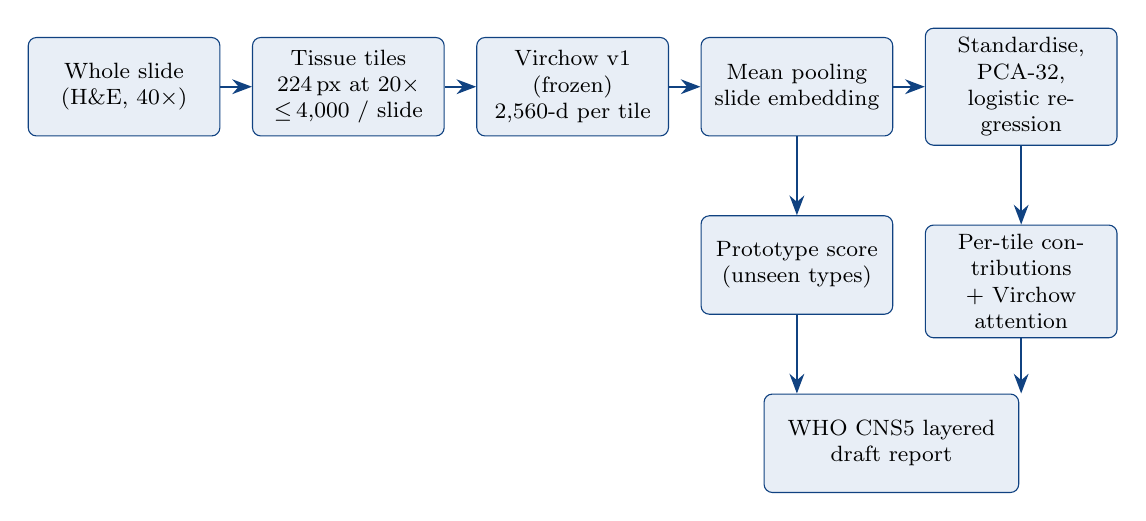
\begin{tikzpicture}[
      box/.style={draw=accent, fill=soft, rounded corners=3pt, align=center, minimum height=1.25cm,
                  text width=2.2cm, font=\footnotesize},
      arr/.style={-{Stealth[length=2.5mm]}, thick, accent}]
    \node[box] (wsi) {Whole slide\\(H\&E, 40$\times$)};
    \node[box, right=0.4cm of wsi] (tile) {Tissue tiles\\224\,px at 20$\times$\\$\le$\,4{,}000 / slide};
    \node[box, right=0.4cm of tile] (vir) {Virchow v1\\(frozen)\\2{,}560-d per tile};
    \node[box, right=0.4cm of vir] (pool) {Mean pooling\\slide embedding};
    \node[box, right=0.4cm of pool] (clf) {Standardise, PCA-32,\\logistic regression};
    \node[box, below=1.0cm of pool] (proto) {Prototype score\\(unseen types)};
    \node[box, below=1.0cm of clf] (exp) {Per-tile contributions\\+ Virchow attention};
    \node[box, below=1.0cm of proto, xshift=1.2cm, text width=3.0cm] (rep) {WHO CNS5 layered\\draft report};
    \draw[arr] (wsi) -- (tile);
    \draw[arr] (tile) -- (vir);
    \draw[arr] (vir) -- (pool);
    \draw[arr] (pool) -- (clf);
    \draw[arr] (pool) -- (proto);
    \draw[arr] (clf) -- (exp);
    \draw[arr] (proto.south) -- (proto.south |- rep.north);
    \draw[arr] (exp.south) -- (exp.south |- rep.north);
  \end{tikzpicture}
  \vspace{0.6em}

  \aside{Feature extraction on a free Kaggle GPU (about 3--4 min per slide); everything after it runs on a laptop CPU.}
\end{frame}

% ------------------------------------------------------------------ evaluation
\begin{frame}{Evaluation protocol}
  \begin{itemize}
    \item \textbf{Known types} (36 slides): leave-one-patient-out. The classifier is refit without the test slide and without any other slide of the same patient.
    \item \textbf{Unseen types}: each rare or held-out type is hidden from training in turn (6 rotations). The detection threshold is set on known slides only, at 95\% of them accepted.
    \item \textbf{Classifier choice}: 12 configurations compared (logistic regression with and without standardisation, PCA, $k$-NN, nearest centroid, linear SVM; mean or mean+max pooling).
  \end{itemize}
  \vspace{0.8em}
  \begin{alertblock}{Caveat}
    42 slides is a feasibility check. Every number below has a wide confidence interval and must be confirmed on new slides.
  \end{alertblock}
\end{frame}

% ------------------------------------------------------------------ classification
\begin{frame}{Result 1: Virchow features separate common and rare types}
  \begin{columns}[c]
    \begin{column}{0.52\textwidth}
      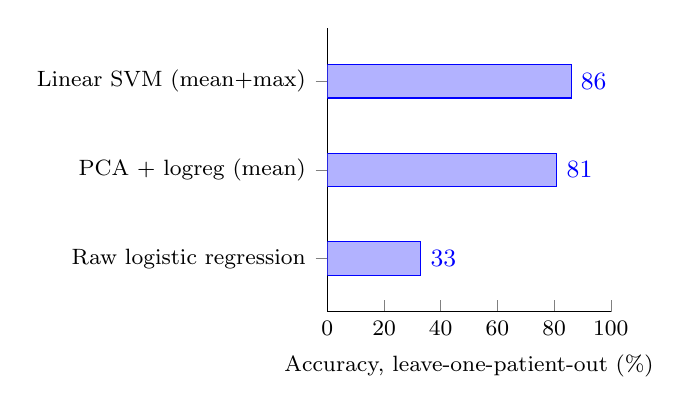
\begin{tikzpicture}
        \begin{axis}[
            xbar, scale only axis, width=3.6cm, height=3.6cm, xmin=0, xmax=100,
            xlabel style={font=\footnotesize}, x tick label style={font=\footnotesize},
            xlabel={Accuracy, leave-one-patient-out (\%)},
            symbolic y coords={{Raw logistic regression},{PCA + logreg (mean)},{Linear SVM (mean+max)}},
            ytick=data, y tick label style={font=\footnotesize, align=right},
            nodes near coords, nodes near coords style={font=\small},
            bar width=12pt, enlarge y limits=0.3, axis lines*=left,
            every axis plot/.append style={fill=accent!70, draw=accent}]
          \addplot coordinates {(33,{Raw logistic regression}) (81,{PCA + logreg (mean)}) (86,{Linear SVM (mean+max)})};
        \end{axis}
      \end{tikzpicture}
    \end{column}
    \begin{column}{0.45\textwidth}
      \begin{itemize}
        \item Standardising the features was the key step: 33\% $\rightarrow$ 81\%.
        \item We keep PCA + logistic regression: calibrated probabilities, and linear, so its score splits exactly over tiles.
        \item Per slide: \textbf{29/36} correct; common 18/20, rare 11/16.
        \item Hardest: CNS lymphoma (1/4), confused with glioblastoma.
      \end{itemize}
      \aside{86\% is the best of 12 configurations, hence optimistic.}
    \end{column}
  \end{columns}
\end{frame}

% ------------------------------------------------------------------ open set
\begin{frame}{Result 2: flagging tumour types never seen in training}
  \begin{columns}[c]
    \begin{column}{0.45\textwidth}
      \textbf{Prototype score}: distance from the slide embedding to the closest known-type mean, after per-dimension standardisation.
      \vspace{0.6em}

      \small
      \begin{tabular}{@{}lcc@{}}
        \toprule
        & L2 only & Standardised\\
        \midrule
        AUROC & 0.63 & \textbf{0.83} $\pm$ 0.20\\
        Unseen caught & 18\% & \textbf{50\%}\\
        Known falsely flagged & -- & 2.6\%\\
        \bottomrule
      \end{tabular}
      \vspace{0.4em}

      \aside{Mean over 6 leave-one-type-out rotations; threshold from known slides only.}
    \end{column}
    \begin{column}{0.53\textwidth}
      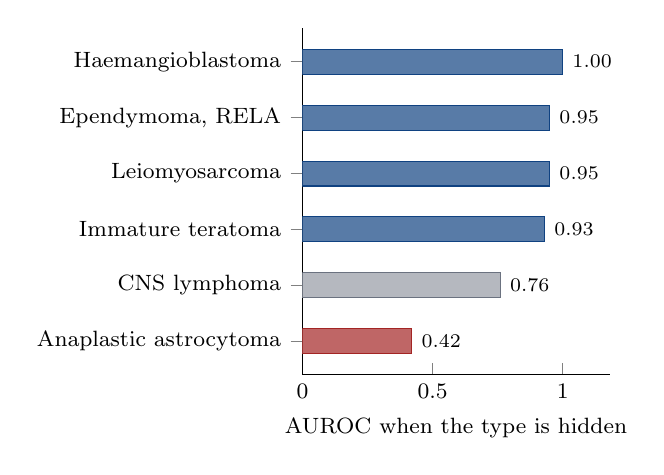
\begin{tikzpicture}
        \begin{axis}[
            xbar, bar shift=0pt, scale only axis, width=3.9cm, height=4.4cm, xmin=0,
            xlabel style={font=\footnotesize}, x tick label style={font=\footnotesize},
            xlabel={AUROC when the type is hidden},
            symbolic y coords={{Anaplastic astrocytoma},{CNS lymphoma},{Immature teratoma},{Leiomyosarcoma},{Ependymoma, RELA},{Haemangioblastoma}},
            ytick={{Anaplastic astrocytoma},{CNS lymphoma},{Immature teratoma},{Leiomyosarcoma},{Ependymoma, RELA},{Haemangioblastoma}},
            y tick label style={font=\footnotesize}, xmax=1.18,
            nodes near coords, nodes near coords style={font=\scriptsize, anchor=west},
            point meta=explicit symbolic,
            bar width=9pt, enlarge y limits=0.12, axis lines*=left]
          \addplot[fill=accent!70, draw=accent] coordinates {
            (1.00,{Haemangioblastoma}) [1.00]
            (0.95,{Ependymoma, RELA}) [0.95]
            (0.95,{Leiomyosarcoma}) [0.95]
            (0.93,{Immature teratoma}) [0.93]};
          \addplot[fill=muted!50, draw=muted] coordinates {(0.76,{CNS lymphoma}) [0.76]};
          \addplot[fill=warm!70, draw=warm] coordinates {(0.42,{Anaplastic astrocytoma}) [0.42]};
        \end{axis}
      \end{tikzpicture}
    \end{column}
  \end{columns}
\end{frame}

\begin{frame}{Far versus near out-of-distribution}
  \begin{columns}[T]
    \begin{column}{0.48\textwidth}
      \begin{block}{Far OOD: well detected}
        Haemangioblastoma, RELA ependymoma, leiomyosarcoma and immature teratoma look unlike every known type (AUROC $\ge 0.93$).
      \end{block}
      \begin{exampleblock}{Intermediate}
        CNS lymphoma (0.76): partly overlaps glioblastoma, as in the closed-set confusions.
      \end{exampleblock}
    \end{column}
    \begin{column}{0.48\textwidth}
      \begin{alertblock}{Near OOD: not detected}
        Anaplastic astrocytoma, IDH-wt (0.42) sits inside the glioblastoma and pilocytic astrocytoma cloud. None of the five scores we tested (confidence, energy, Mahalanobis, $k$-NN, prototype) separates it.
      \end{alertblock}
      \vspace{0.4em}
      \textbf{Consequence}: report far and near OOD separately; a hierarchical level (``glioma, subtype uncertain'') is a natural next step.
    \end{column}
  \end{columns}
\end{frame}

% ------------------------------------------------------------------ explainability
\begin{frame}{Result 3: which tiles made the call}
  \centering
  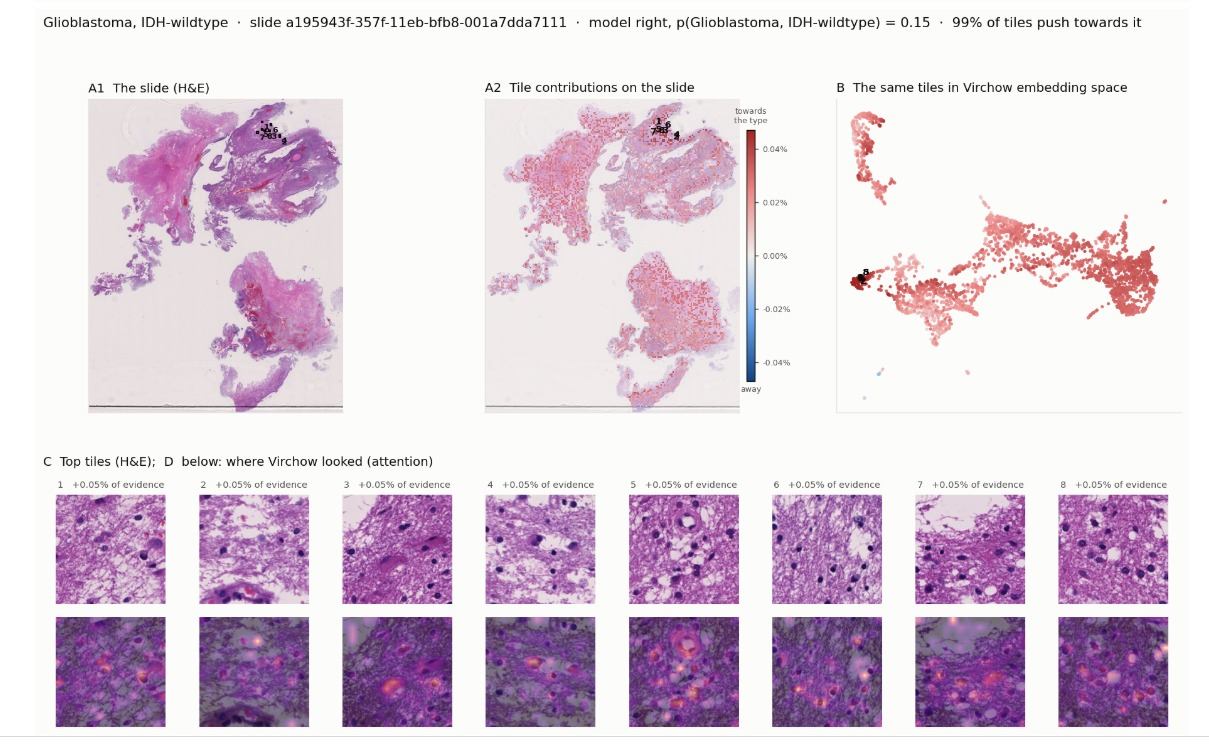
\includegraphics[height=0.66\textheight]{figures/gbm_explanation.jpg}\\[0.2em]
  \raggedright\footnotesize
  Mean of tile embeddings + linear classifier $\Rightarrow$ the score splits exactly over the $n$ tiles,
  $s_c = \sum_i \tfrac{1}{n}(w_c-\bar w)^\top t_i + b_c$: each term is that tile's exact Shapley value.
  A1 slide, A2 contribution map, B tiles in Virchow space, C top H\&E tiles, D Virchow attention.\\
  \aside{Glioblastoma slide; figure from an earlier, unstandardised classifier, hence the low probability.}
\end{frame}

% ------------------------------------------------------------------ PRISM
\begin{frame}{Baseline: PRISM reports from the same Virchow features}
  \begin{columns}[T]
    \begin{column}{0.5\textwidth}
      \small
      \begin{tabular}{@{}lc@{}}
        \toprule
        Tumour type & Type named correctly\\
        \midrule
        Pituitary adenoma & 5/5\\
        Pilocytic astrocytoma & 4/5\\
        CNS lymphoma & 4/4\\
        Leiomyosarcoma & 4/4 (as sarcoma)\\
        Glioblastoma, IDH-wt & 2/5\\
        Haemangioblastoma & 2/3\\
        Ependymoma, RELA & 1/4\\
        Meningothelial meningioma & 0/5\\
        Immature teratoma & 0/4\\
        Anaplastic astrocytoma & 0/3\\
        \midrule
        \textbf{Total} & \textbf{about 22/42}\\
        \bottomrule
      \end{tabular}
    \end{column}
    \begin{column}{0.47\textwidth}
      \begin{itemize}
        \item Good on visually distinctive types; never names meningioma.
        \item Reaches for diagnoses from outside the brain (sarcoma, GIST, carcinoma).
        \item \alert{Makes up findings}: wrong organ (lymph node, uterus), immunostains and Ki-67 that H\&E cannot show.
        \item One fluent line, not a structured report.
      \end{itemize}
      \aside{Graded by the authors, not yet by a neuropathologist.}
    \end{column}
  \end{columns}
\end{frame}

% ------------------------------------------------------------------ report
\begin{frame}{Result 4: evidence-grounded WHO CNS5 draft reports}
  \begin{columns}[T]
    \begin{column}{0.5\textwidth}
      Layered format of the ICCR dataset, every field filled from facts the pipeline can show:
      \begin{itemize}
        \item \textbf{Integrated diagnosis}: type, given as NOS because molecular status is unknown
        \item \textbf{Histopathological classification} and \textbf{CNS WHO grade}
        \item \textbf{Molecular information}: ``not assessed'', with the tests to request
        \item \textbf{Microscopic findings}: probability, tiles analysed
        \item \textbf{Comment}: differential and coordinates of the regions to review
      \end{itemize}
    \end{column}
    \begin{column}{0.47\textwidth}
      \begin{block}{Safety rules}
        \begin{itemize}
          \item Below $p = 0.5$: ``Indeterminate on H\&E'' with a differential.
          \item Above the prototype threshold: ``tumour type not recognised by the model'', with methylation profiling suggested.
          \item An optional LLM may rephrase findings, but its text is rejected if it contradicts the diagnosis.
        \end{itemize}
      \end{block}
      \aside{Every report is marked as a research draft.}
    \end{column}
  \end{columns}
\end{frame}

% ------------------------------------------------------------------ limits
\begin{frame}{Limitations}
  \begin{itemize}
    \item \textbf{Small sample}: 42 slides, 3--5 per type; confidence intervals are wide.
    \item \textbf{Optimistic selection}: the classifier was chosen on the same slides it was scored on.
    \item \textbf{Ten types only}, out of 126 in the atlas.
    \item \textbf{No expert review yet}: PRISM grading and the WHO mapping table need a neuropathologist.
    \item \textbf{H\&E only}: IDH, fusions and methylation class, central to WHO CNS5, are out of reach.
    \item \textbf{Single magnification} (20$\times$), at most 4{,}000 tiles per slide.
  \end{itemize}
\end{frame}

% ------------------------------------------------------------------ next
\begin{frame}{Next steps}
  \begin{columns}[T]
    \begin{column}{0.48\textwidth}
      \textbf{Data and models}
      \begin{itemize}
        \item 15--20 slides per type, more rare types
        \item Attention-based MIL pooling (ABMIL)
        \item Multi-magnification features
        \item Hierarchical labels for near-OOD gliomas
      \end{itemize}
    \end{column}
    \begin{column}{0.48\textwidth}
      \textbf{Evaluation}
      \begin{itemize}
        \item Confirm accuracy and AUROC on new, untouched slides
        \item Report far and near OOD separately
        \item Neuropathologist rating of reports: correctness and made-up findings, ours vs PRISM
      \end{itemize}
    \end{column}
  \end{columns}
\end{frame}

% ------------------------------------------------------------------ takeaways
\begin{frame}{Take-aways}
  \begin{enumerate}
    \item Frozen Virchow v1 features, standardised, recognise common \emph{and} rare brain tumour types in a 42-slide pilot (29/36 slides, leave-one-patient-out).
    \item A standardised prototype score flags clearly different unseen types (AUROC $\ge$ 0.93) but not near-OOD gliomas.
    \item A linear classifier on mean-pooled tiles gives exact, cheap per-tile explanations.
    \item Structured WHO CNS5 reports state only what this evidence supports; PRISM, on the same features, makes up organs and stains. Expert rating is the next test.
  \end{enumerate}
  \vspace{1em}
  \centering
  {\color{muted}Code: \texttt{github.com/AsmaActiveLearning/Cancer\_diagnosis}}
\end{frame}

\begin{frame}[plain]
  \centering
  \vfill
  {\Huge\color{accent} Thank you}\\[1em]
  Asma Baghdadi \quad Aymen Ben Brik\\[0.5em]
  {\color{muted}\small Data: EBRAINS Digital Brain Tumour Atlas (Roetzer-Pejrimovsky et al., 2022).\\
  Models: Virchow v1 and PRISM (Paige), research use only.}
  \vfill
\end{frame}

\end{document}
